% !TEX program = xelatex

\documentclass{resume}
\usepackage{zh_CN-Adobefonts_external} % Simplified Chinese Support using external fonts (./fonts/zh_CN-Adobe/)
\usepackage{graphicx}
\usepackage{tabu}
\usepackage{multirow}
\usepackage{progressbar}
%\usepackage{zh_CN-Adobefonts_external} % Simplified Chinese Support using external fonts (./fonts/zh_CN-Adobe/)
%\usepackage{zh_CN-Adobefonts_internal} % Simplified Chinese Support using system fonts

\begin{document}
\pagenumbering{gobble} % suppress displaying page number

\Large{
  \begin{tabu}{ c l r }
   \multirow{5}{1in}{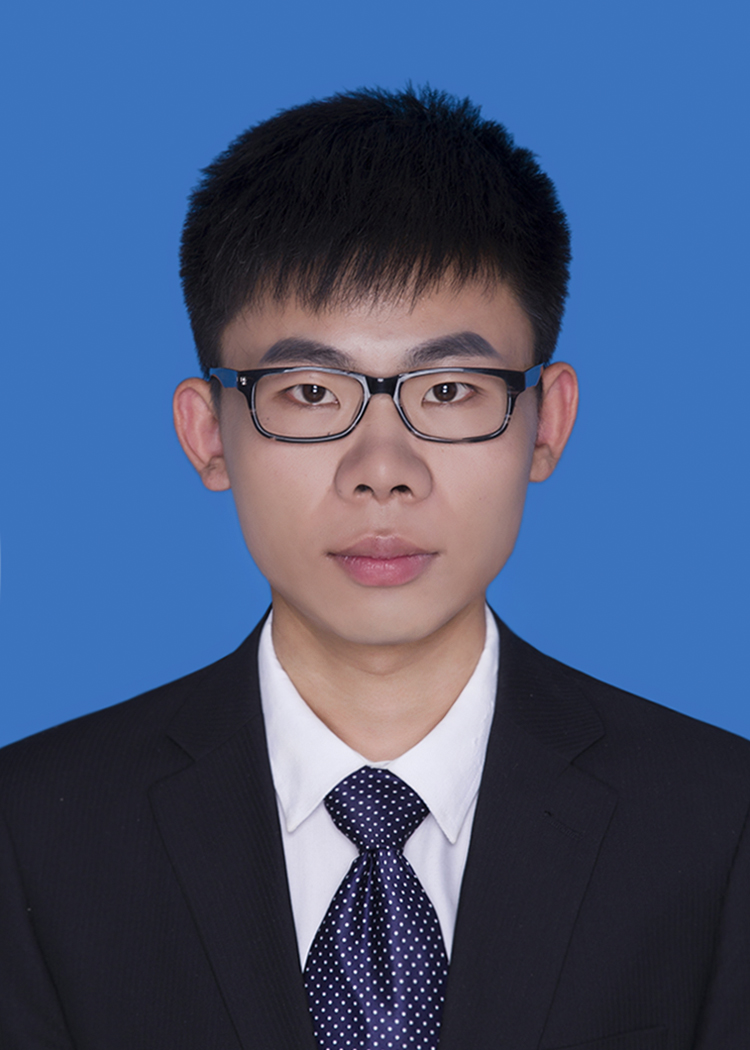
\includegraphics[width=0.88in]{ezra}} & \scshape{侯传浩} & {C++~}\progressbar{0.75} \\
    & \email{houchuanhao@imudges.com} & {Verilog~}\progressbar{0.5} \\
    & \phone{(+86) 18800235950} & {Linux~}\progressbar{0.5} \\
    & \location{上海科技大学}& {Python~}\progressbar{0.7} \\
    &年龄:28 & {Perl~}\progressbar{0.6}\\
    &兴趣爱好:马拉松、健身 & 
  \end{tabu}
}

\section{\faGraduationCap\  教育背景}


\datedsubsection{\textbf{上海科技大学} ~~\textit{硕士}~~\ 计算机科学与技术}{2020.9 —— 2024.6}
\datedsubsection{主修课程:数字集成电路 、计算机体系结构、深度学习}{}
\datedsubsection{\textbf{内蒙古大学}  \ \ \ \ \ ~~\textit{本科}~~\ 软件工程}{2014.9——2018.6}
\datedsubsection{主修课程:算法与数据结构、计算机组成原理、计算机操作系统、计算机网络、编译原理}{}
%\datedsubsection{获奖经历}

\datedsubsection{}{}
\section{\faUsers\ 专业技能}

\datedsubsection{\textbf{1.} 熟练掌握C++ 、python 、perl 语言 }{}
\datedsubsection{\textbf{4.}  熟悉PCI 、SATA、AHCI 、ESPI 等协议标准,熟悉verilog以及芯片设计开发流程}{}
\datedsubsection{\textbf{5.}  熟悉SSD 基本结构及运行机制 }{}
\datedsubsection{\textbf{2.}  熟悉计算机体系结构}{}
\datedsubsection{\textbf{3.}  熟悉符号执行基本原理 }{}
\datedsubsection{\textbf{6.}  熟练掌握常用深度学习算法,了解基本的神经网络模型}{}
\datedsubsection{\textbf{7.}  熟练掌握常用算法及数据结构}{}
\datedsubsection{\textbf{8.}  熟练掌握git}{}

\datedsubsection{}{}


\section{\faUsers\ 实习/项目经历}

\datedsubsection{\textbf{上海兆芯集成电路有限公司}  ~~\textit{ASIC设计(实习)}~~\ 负责兆芯某处理器项目南桥芯片组ESPI模块的debug}{2021.9——2023.3}
\datedsubsection{\textbf{上海科技大学}  ~~\textit{课程设计}~~\ 小型卷积核电路设计}{2021.3——2021.6}
\datedsubsection{\textbf{华为技术有限公司北京研究所}  ~~\textit{软件工程师}~~\  负责华为5G云核心网项目的开发和维护  }{2020.5——2020.8}
\datedsubsection{\textbf{北京轩宇信息科技有限公司}  ~~\textit{软件工程师}~~\ 负责一款基于符号执行的自动化软件测试工具
的研发}{2019.1——2019.7}
\datedsubsection{\textbf{北京开心人信息技术有限公司}  ~~\textit{软件工程师}~~\ 游戏开发}{2018.7——2018.11}
\datedsubsection{}{}

\section{\faUsers\ 获奖经历}

\datedsubsection{\textbf{内蒙古自治区程序设计大赛}  ~~\textit{三等奖}~~\ }{2016}
\datedsubsection{\textbf{内蒙古自治区程序设计大赛}  ~~\textit{三等奖}~~\ }{2015}
\datedsubsection{\textbf{第二届内蒙古自治区“互联网+”大学生创新创业大赛银奖}  ~~\textit{银奖}~~\ }{2016}
\datedsubsection{\textbf{华北五省计算机应用大赛三等奖}  ~~\textit{三等奖}~~\ }{2016}
% Reference Test
%\datedsubsection{\textbf{Paper Title\cite{zaharia2012resilient}}}{May. 2015}
%An xxx optimized for xxx\cite{verma2015large}
%\begin{itemize}
%  \item main contribution
%\end{itemize}

% \section{\faCogs\ Skills}
% \begin{itemize}[parsep=0.5ex]
%   \item Programming Languages: C == Python > C++ > Java
%   \item Platform: Linux
%   \item Development: Web, xxx
% \end{itemize}

% \section{\faHeartO\ Honors and Awards}
% \datedline{\textit{\nth{1} Prize}, Award on xxx }{Jun. 2013}
% \datedline{Other awards}{2015}



%% Reference
%\newpage
%\bibliographystyle{IEEETran}
%\bibliography{mycite}
\end{document}
